\chapter{METODOLOGÍA}
Debido a que las metodologías de software nacen para ordenar y promover buenas prácticas en el desarrollo de software de calidad, actualmente se encuentran numerosos modelos y metodologías que se pueden adaptar dependiendo las necesidades del producto final a entregar,\parencite{Nohemy2015ESCOGERDECISION} para el proyecto “NOMBRE DEL PROYECTO” se determinaron perspectivas importantes para la selección de la metodología adecuada, empezado por una metodología que permita el desarrollo de forma ágil, debido a que es un proyecto estipulado a 6 meses, necesita una verificación diaria durante todo su ciclo de vida que permita un crecimiento preciso y controlado, que se tomen decisiones rápidas y adaptables acorde al desarrollo de la aplicación. 


Antes de comenzar es necesario definir el producto, el equipo de SCRUM y las tareas generales a realizar, para sí elaborar la estructura del proyecto con la metodología, el equipo de trabajo estará compuesto así: 
\begin{itemize}
    \item Product Owner:  Con el objetivo de tener varios puntos de vista, hemos conseguido un grupo de profesionales que nos permiten tener una visión interdisciplinar para cumplirán este rol.
    \begin{enumerate}
        \item Diana Rivera Castillo, Ingeniera industrial con especialización en salud ocupacional, Youtuber Colombiana más influyente en Salud y seguridad en el trabajo SST, y actual Gerente de HSEQ Nueva Visión.
        \item Jorge Enrique Moreno Collazos, Fisioterapeuta, especialista en rehabilitación Cardiopulmonar, magíster en ciencias de la actividad física y el deporte, magíster en calidad educativa, doctor en salud pública, doctor en terapia manual, doctor en educación, Pos doctorado en educación, ciencias sociales e interculturalidad. Docente e investigador.
        \item Ximena Cano, Médica de la Universidad de Ciencias Aplicadas y Ambientales U.D.C.A. 
    \end{enumerate}

\item Scrum Master: esté cargo estará ocupado por Daniel Nieto Gomez.
\item Equipo desarrollador: Estará compuesto por Junior Parra como desarrollador de Scripting en Back end C\# y análisis de software, junto con Daniel Nieto Gómez como diseñador y desarrollador Front end y Análisis enfocado en el uso de herramientas de IA (inteligencia artificial). 
\end{itemize}

La duración del Sprint quedará cada semana y media, por el periodo correspondiente al proyecto que es de 6 meses.

Por tratarse de un producto de software, una de las primeras tareas que se deben iniciar es la ingeniería de requerimientos o levantamiento de requerimientos, escribir los casos de uso más importantes y discutirlos con los product owners y  partes interesadas, luego de recopilar los casos de uso y los requisitos de alto nivel, se escriben en el SCRUM product Backlog y se inicia la estimación y priorización de las sesiones con el equipo SCRUM, Luego se comienzan a dividir los requerimientos de alto nivel en requerimientos más pequeños, que se puedan enmarcar en historias de usuario, con esta lista se convoca a la reunión de planeación del primer Sprint (Sprint planning meetting).

\begin{figure}[H]
    \centering
    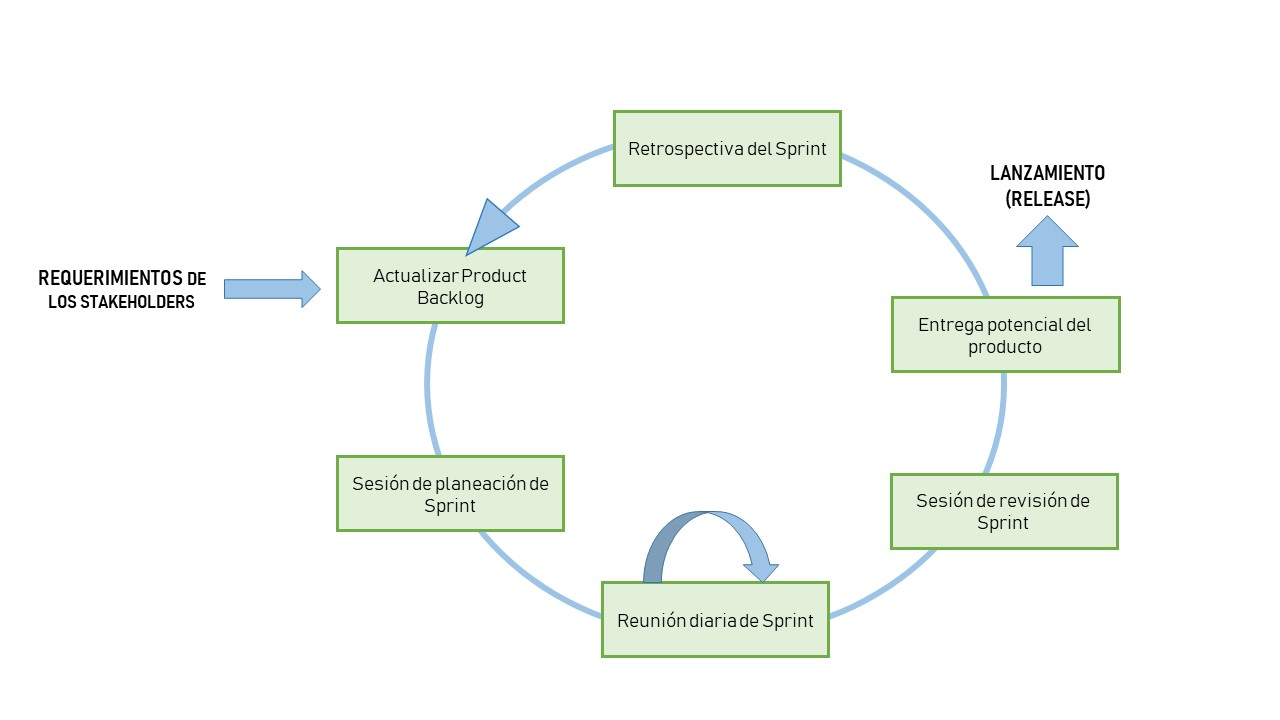
\includegraphics[width=1\textwidth]{Anexos/LATEX/chapters/images/Scrum_1.jpg}
    \caption{Diagrama de Fases y Sprints para el proyecto}
    \small{\textbf{Fuente:} Elaboración propia}
    \label{SCRUM2}
\end{figure}

Para el correcto almacenamiento de la aplicación y documentación, debido a que la periodicidad es diaria, se utilizará GitHub, para cada Sprint diario y versionamiento.    


 

